\subsection{Augmentation, our results}

\begin{figure}[H]
\center
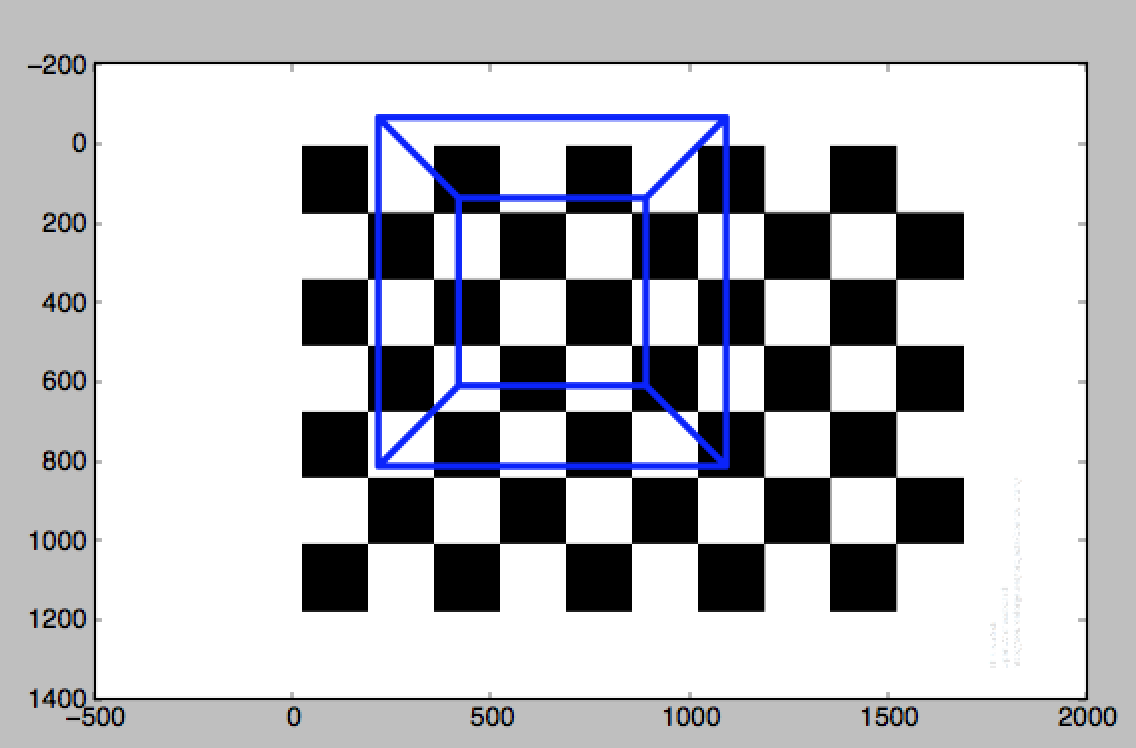
\includegraphics{pics/result0.png}
\caption{Our first projection onto the pattern image. The perspective projection effect is very visable on this image. Notice the translation of the pattern. This will affect the placement of the box on the rest of the images.}
\label{result0}
\end{figure}

\begin{figure}[H]
\center
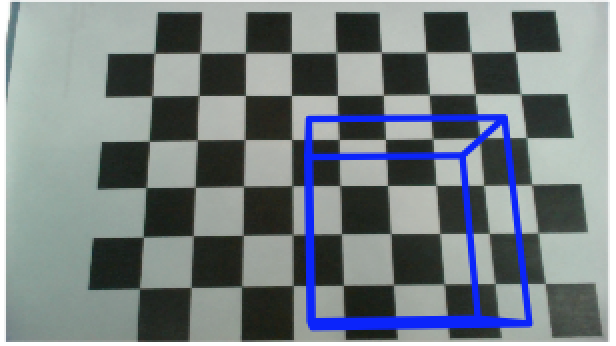
\includegraphics{pics/result1.png}
\caption{On this image the chessboard is only moved slightly away from the full frontal position. The position of the boc on the pattern doesn’t correspond to the position of the pattern image, but is consistent with the rest of the images.}
\label{result1}
\end{figure}

\begin{figure}[H]
\center
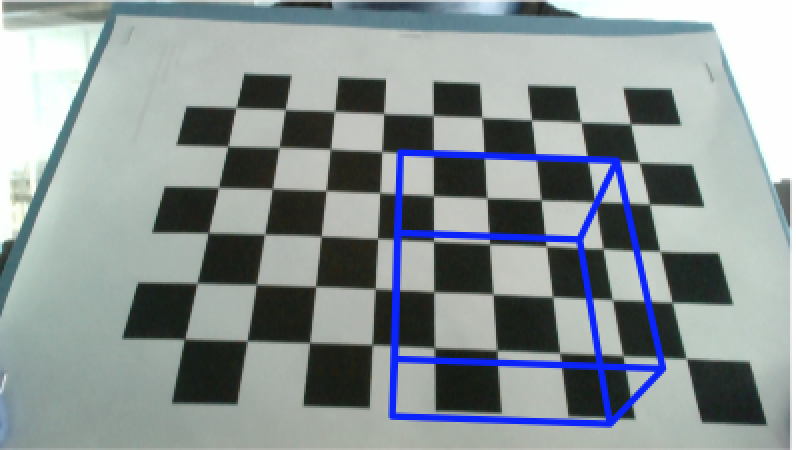
\includegraphics{pics/result2.png}
\caption{The 3d effect gets more pronounced as the chessboard is moved further away from the frontal position. The box doesn’t look completely even, but that is caused by the estimation of the z axis.}
\label{result2}
\end{figure}

\begin{figure}[H]
\center
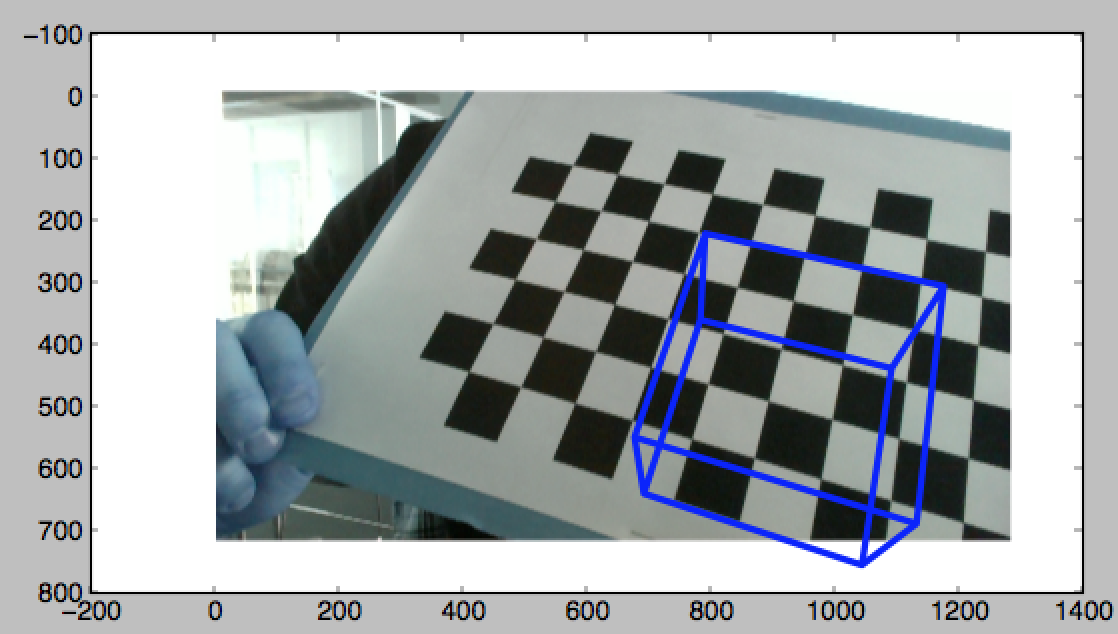
\includegraphics{pics/result3.png}
\caption{As we see here. The projection and plotting of the box, doesn’t care about image limits in this implementation. Gives a pretty nice effect though. (Best viewed with 3d glasses :-))}
\label{result3}
\end{figure}


\begin{figure}[H]
\center
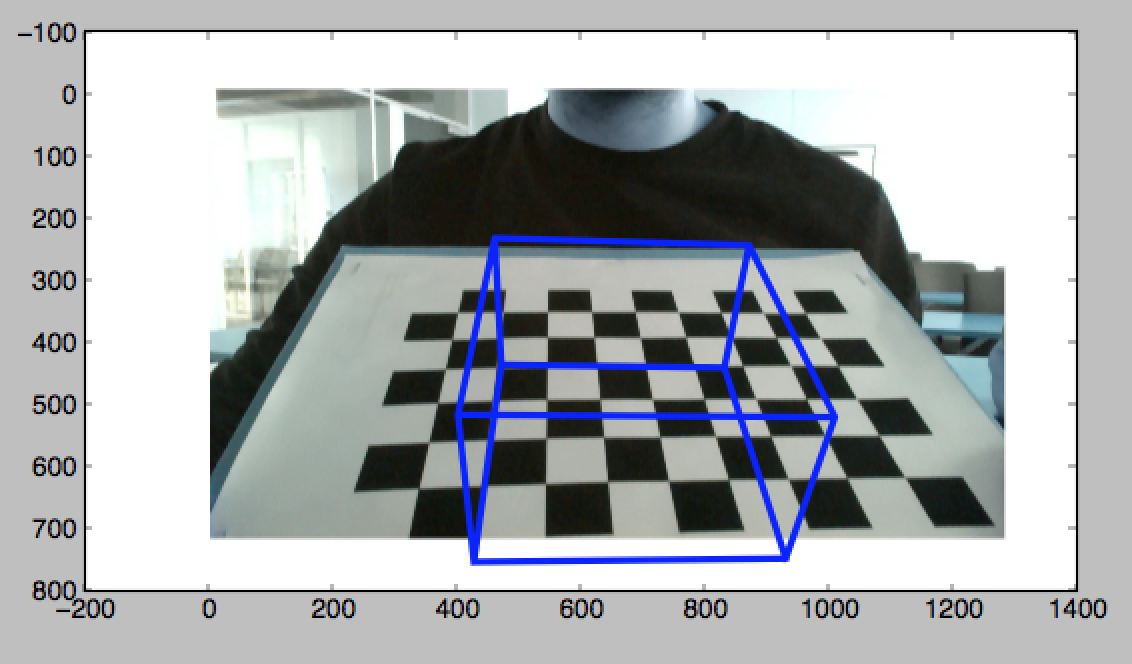
\includegraphics{pics/result4.png}
\caption{The augmentation effect works best when the surroundings are visible. Also note that the box looks a bit skewed/uneven but follows the chessboard pattern exactly because of the homography.}
\label{result4}
\end{figure}

\begin{figure}[H]
\center
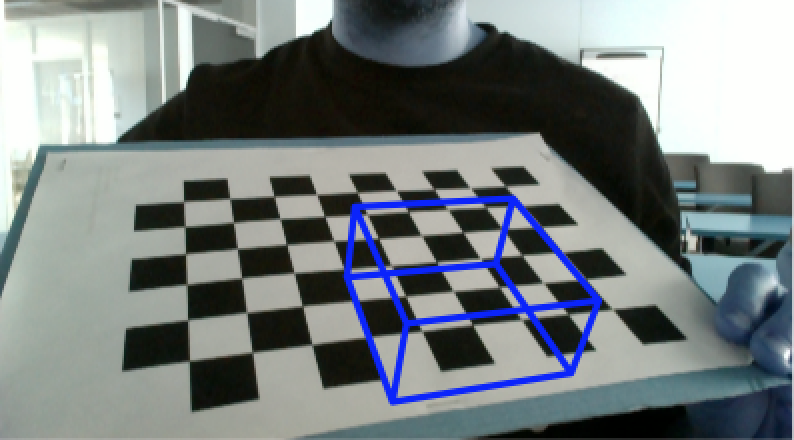
\includegraphics{pics/result5.png}
\caption{Last image. Lets just notice that it looks awesome. Next stop cool 3d models projected on family photos.}
\label{result5}
\end{figure}
